\documentclass{standalone}

\usepackage{tikz}
\usepackage{xcolor}
\definecolor{primary}{HTML}{003262} % berkeley blue
\definecolor{secondary}{HTML}{FDB515} % cal gold
\definecolor{founder}{HTML}{3B7EA1}
\definecolor{medalist}{HTML}{C4820E}
\definecolor{goldengate}{HTML}{ED4E33}
\definecolor{ion}{HTML}{CFDD45}

\begin{document}
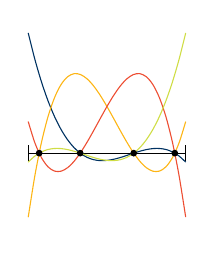
\begin{tikzpicture}
	% \tikzset{shift=(current page.center), xshift=-4cm, yshift=-3.75cm}
	\scriptsize
	\draw (-1,0) -- (1,0); 
	\draw (-1,-.1) -- (-1,.1); 
	\draw (1,-.1) -- (1,.1); 
	\draw[domain=-1:1, smooth, primary] plot 
		(\x, -0.92756751*\x*\x*\x + 0.79876206*\x*\x + 0.10721485*\x - 0.0923266); 
	\draw[domain=-1:1, smooth, secondary] plot 
		(\x, 2.34943118*\x*\x*\x -0.79876206*\x*\x -1.74223419*\x + 0.5923266); 
	\draw[domain=-1:1, smooth, goldengate] plot 
		(\x, -2.34943118*\x*\x*\x -0.79876206*\x*\x + 1.74223419*\x + 0.5923266); 
	\draw[domain=-1:1, smooth, ion] plot
		(\x, 0.92756751*\x*\x*\x + 0.79876206*\x*\x -0.10721485*\x -0.0923266); 
	\foreach \x in {-0.86113631, -0.33998104,  0.33998104,  0.86113631}{
		\filldraw[black] (\x,0) circle[radius=1pt]; 
	}
	\node at (0,-.85) {}; 
	\node at (0,1.5) {}; 
\end{tikzpicture}
\end{document}